% ===== SECTION 1: PREAMBLE AND TITLE SETUP =====
\documentclass[11pt,twoside]{article}

% Essential packages
\usepackage[utf8]{inputenc}
\usepackage[T1]{fontenc}
\usepackage[english]{babel}
\usepackage{geometry}
\usepackage{fancyhdr}
\usepackage{titlesec}
\usepackage{authblk}
\usepackage{setspace}
\usepackage{parskip}
\usepackage{microtype}
\usepackage{xcolor}
\usepackage{amsmath}
\usepackage{amsfonts}
\usepackage{csquotes}
\usepackage{longtable}
\usepackage{enumitem}
\usepackage{xspace}
\usepackage{tikz}
\usetikzlibrary{arrows.meta,positioning,fit,shapes.geometric}

% Journal-style formatting
\geometry{
  paper=letterpaper,
  margin=0.4in,
  marginparwidth=0.4in,
  marginparsep=0.4in
}

% Define colors
\definecolor{darkblue}{RGB}{0,73,144}
\definecolor{mediumgray}{RGB}{64,64,64}
\definecolor{systemicred}{RGB}{231,76,60}

% Fairness metric helpers — text-safe (no math mode required)
\DeclareRobustCommand{\EOgap}{EO\text{-}gap\xspace}
\DeclareRobustCommand{\TPR}{TPR\xspace}
\DeclareRobustCommand{\FNR}{FNR\xspace}
\DeclareRobustCommand{\ECE}{ECE\xspace}
\DeclareRobustCommand{\pp}{pp\xspace} % percentage points

% Section formatting
\titleformat{\section}
  {\normalfont\large\bfseries\color{darkblue}}{\thesection}{1em}{}
\titleformat{\subsection}
  {\normalfont\normalsize\bfseries\color{mediumgray}}{\thesubsection}{1em}{}
\titleformat{\subsubsection}
  {\normalfont\small\bfseries\color{mediumgray}}{\thesubsubsection}{1em}{}

% Header and footer
\pagestyle{fancy}
\fancyhf{}
\fancyhead[LE]{\small\textcolor{mediumgray}{\textit{IDAI700 Portfolio}}}
\fancyhead[RO]{\small\textcolor{mediumgray}{\textit{From Harm to Equity}}}
\fancyfoot[C]{\thepage}
\renewcommand{\headrulewidth}{0.5pt}
\renewcommand{\footrulewidth}{0pt}

% Hyperlink setup (load LAST)
\usepackage{hyperref}
\urlstyle{same}

\hypersetup{
  breaklinks=true,
  colorlinks=true,
  linkcolor=darkblue,
  citecolor=darkblue,
  urlcolor=darkblue,
  pdftitle={EQUITAS: A Lived Journey to Ethical AI for CLD Diagnostics},
  pdfauthor={Piter Garcia},
  pdfsubject={IDAI700 Portfolio Narrative},
  pdfkeywords={AI ethics, EQUITAS framework, CLD youth, fairness metrics, systemic bias, lived experience}
}

% Title formatting
\title{
\vspace*{1.5in}
\textbf{\Huge EQUITAS: A Lived Journey to Ethical AI}\\[0.5em]
\Large Systemic Harm, Personal Survival, and Community Repair in CLD Diagnostics\\[1.5em]
\large IDAI700 Portfolio Narrative --- Scholarly Synthesis Through Lived Authority\\[2em]

\vfill
\Large \textbf{Piter Garcia}\\
\normalsize IDAI700: Ethics of Artificial Intelligence\\
Rochester Institute of Technology\\
\texttt{pzg8794@rit.edu}\\[1em]

\large \textbf{November 12, 2025}\\
\normalsize \textit{Thinking Process Documentation \& EQUITAS Framework Development}
}
\author{}
\date{}

\sloppy
\begin{document}
\thispagestyle{empty}
\maketitle

\vspace{0.5in}
\noindent\textit{\tiny\textbf{Academic Integration Statement:} 
This IDAI700 (AI Ethics) research portfolio synthesizes core ethics readings with insights from ED415 (Adolescent Development and Youth Culture) at the University of Rochester; the \textbf{Puzzle Plan}---an interdisciplinary, modular research framework that fuses computational methods, educational equity, and lived experience to build equitable diagnostic systems and translate findings into tools, policy, and pedagogy; and the \textbf{EQUITAS} framework (Equity-Queried Universal Insights for Transparent Algorithmic Systems), an ethical checklist for fairness-aware machine learning in health screening. Together, these tools argue that \emph{diagnostic equity requires relational assessment, ecological contextualization, and community-partnered design} in AI-driven screening systems, with implications for school-based social-emotional assessment, peer-relationship evaluation, and family-centered diagnostic protocols in underserved communities.}
\newpage
\pagestyle{fancy}


% ===== Abstract =====
\section*{Portfolio Narrative: From Lived Harm to Verifiable Trust}
\noindent This portfolio narrates a journey across seven entries, tracing the arc from lived harm and diagnostic erasure in AI systems to a verifiable framework for equity through human-AI partnership. Guided by my Puzzle Plan's interdisciplinary modular design, the EQUITAS framework unfolds in layered progression: beginning with \textbf{co-design} (Entry~1)---the foundational interdisciplinary layer that centers community voices in AI development; advancing to \textbf{governance} (Entry~2)---the policy and enforcement layer ensuring accountability; building toward \textbf{civic literacies} (Entry~3)---the vital space where diverse truths are voiced and validated, strengthened by \textbf{trust as evidence} (Entry~4)---a transparency-driven layer that fosters reliability; then addressing \textbf{empirical disparities} (Entry~5)---the human-centered layer that combats isolation by illuminating overlooked inequities; and culminating in \textbf{metrics and procedures} (Entry~6)---the integrative layer that connects all pieces through accessible fairness metrics and participatory protocols, yielding insights into long-unresolved disparities and events.


% ===== EQUITAS Framework Diagram (Layered Progression) =====
\vspace{0.2cm}
\begin{center}
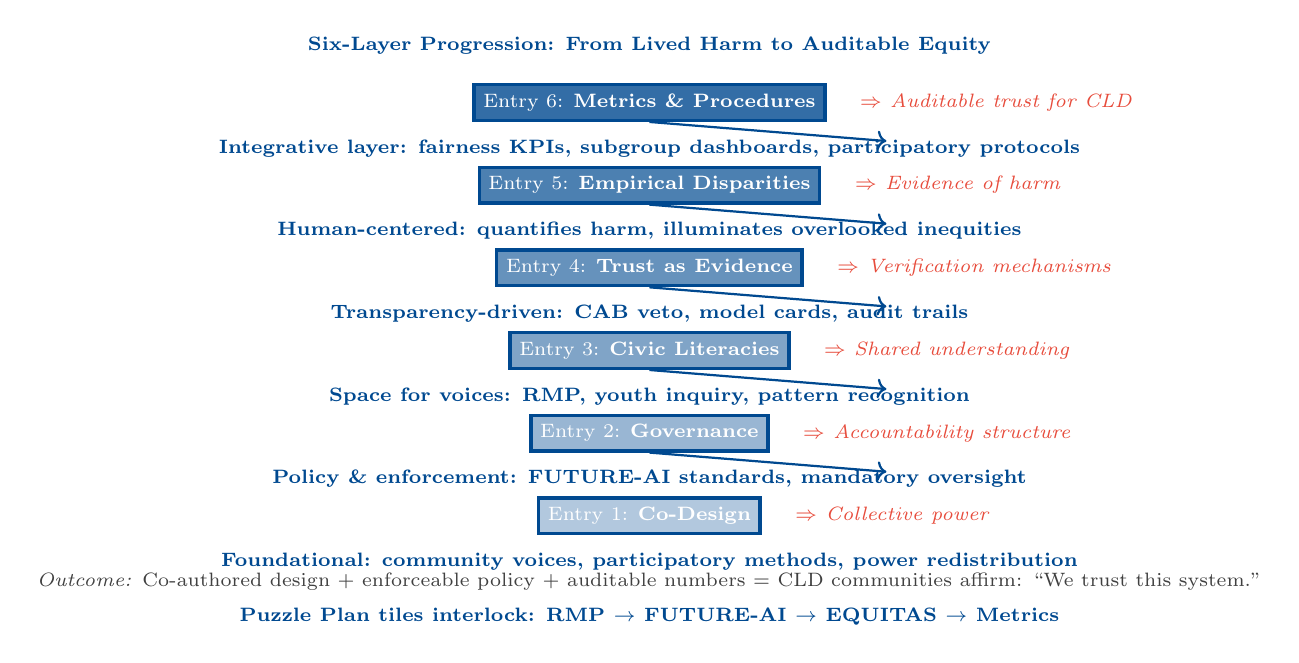
\begin{tikzpicture}[
  scale=0.7,
  node distance=0.8cm,
  every node/.style={font=\scriptsize, text centered},
  layer/.style={rectangle, minimum width=1cm, minimum height=0.1cm, draw=darkblue, very thick, text=white, fill=darkblue!80},
  label_style/.style={font=\scriptsize\bfseries, text=darkblue},
  arrow/.style={->, thick, darkblue}
]

% Title
\node[font=\scriptsize\bfseries\color{darkblue}, anchor=south] at (3.5, 9.2) {Six-Layer Progression: From Lived Harm to Auditable Equity};

% Layer 6: Metrics & Procedures (top)
\node[layer] (E6) at (3.5, 8.5) {Entry 6: \textbf{Metrics \& Procedures}};
\node[label_style, below=0.1cm of E6] {\scriptsize Integrative layer: fairness KPIs, subgroup dashboards, participatory protocols};

% Arrow down
\draw[arrow] (E6.south) -- (7.8, 7.8);

% Layer 5: Empirical Disparities
\node[layer, fill=darkblue!70] (E5) at (3.5, 7) {Entry 5: \textbf{Empirical Disparities}};
\node[label_style, below=0.1cm of E5] {\scriptsize Human-centered: quantifies harm, illuminates overlooked inequities};

% Arrow down
\draw[arrow] (E5.south) -- (7.8, 6.3);

% Layer 4: Trust as Evidence
\node[layer, fill=darkblue!60] (E4) at (3.5, 5.5) {Entry 4: \textbf{Trust as Evidence}};
\node[label_style, below=0.1cm of E4] {\scriptsize Transparency-driven: CAB veto, model cards, audit trails};

% Arrow down
\draw[arrow] (E4.south) -- (7.8, 4.8);

% Layer 3: Civic Literacies
\node[layer, fill=darkblue!50] (E3) at (3.5, 4) {Entry 3: \textbf{Civic Literacies}};
\node[label_style, below=0.1cm of E3] {\scriptsize Space for voices: RMP, youth inquiry, pattern recognition};

% Arrow down
\draw[arrow] (E3.south) -- (7.8, 3.3);

% Layer 2: Governance
\node[layer, fill=darkblue!40] (E2) at (3.5, 2.5) {Entry 2: \textbf{Governance}};
\node[label_style, below=0.1cm of E2] {\scriptsize Policy \& enforcement: FUTURE-AI standards, mandatory oversight};

% Arrow down
\draw[arrow] (E2.south) -- (7.8, 1.8);

% Layer 1: Co-Design (foundation)
\node[layer, fill=darkblue!30] (E1) at (3.5, 1) {Entry 1: \textbf{Co-Design}};
\node[label_style, below=0.1cm of E1] {\scriptsize Foundational: community voices, participatory methods, power redistribution};

% Right-side annotations (Context/Outcome)
\node[font=\scriptsize\itshape\color{systemicred}, right=0.3cm of E6, anchor=west] {$\Rightarrow$ Auditable trust for CLD};
\node[font=\scriptsize\itshape\color{systemicred}, right=0.3cm of E5, anchor=west] {$\Rightarrow$ Evidence of harm};
\node[font=\scriptsize\itshape\color{systemicred}, right=0.3cm of E4, anchor=west] {$\Rightarrow$ Verification mechanisms};
\node[font=\scriptsize\itshape\color{systemicred}, right=0.3cm of E3, anchor=west] {$\Rightarrow$ Shared understanding};
\node[font=\scriptsize\itshape\color{systemicred}, right=0.3cm of E2, anchor=west] {$\Rightarrow$ Accountability structure};
\node[font=\scriptsize\itshape\color{systemicred}, right=0.3cm of E1, anchor=west] {$\Rightarrow$ Collective power};

% Bottom synthesis
\node[font=\scriptsize\bfseries, text=darkblue, below=0.8cm of E1] 
  {Puzzle Plan tiles interlock: RMP $\rightarrow$ FUTURE-AI $\rightarrow$ EQUITAS $\rightarrow$ Metrics};
\node[font=\scriptsize, text=mediumgray, below=0.35cm of E1] 
  {\textit{Outcome:} Co-authored design + enforceable policy + auditable numbers = CLD communities affirm: ``We trust this system.''};

\end{tikzpicture}
\end{center}
\vspace{-0.5cm}
\noindent {\tiny\textbf{Key Metrics:} $\mathrm{EO\text{-}gap} \le 3\,\pp$ (equalized odds parity), $\mathrm{TPR\text{-}ratio} \in [0.9,1.1]$ (sensitivity equity), $\mathrm{ECE}_{\text{subgroup}} \le 0.03$ (calibration per group).}
% ===== END DIAGRAM =====

\vspace{0.2cm}
\noindent \textsc{EQUITAS}---\textit{Equity-Centered, Universal, Traceable, Usable, Robust, Explainable}---operationalizes the cover-page claim that diagnostic equity requires \emph{relational assessment}, \emph{ecological contextualization}, and \emph{community-partnered design}. In practice, it runs a co-design $\rightarrow$ governance $\rightarrow$ metrics pipeline that embeds family--school--clinic context, empowers Community Advisory Boards (CABs) with veto authority, and uses subgroup KPIs to make trust auditable in CLD communities: $\mathrm{EO\text{-}gap} \le 3\,\pp$, $\mathrm{TPR\text{-}ratio} \in [0.9,1.1]$, and $\mathrm{ECE}_{\text{subgroup}} \le 0.03$.

\vspace{0.2cm}
\noindent Within the \textit{Puzzle Plan}---an interdisciplinary framework that fuses computational methods, educational equity, and lived experience---\textsc{EQUITAS} is the fairness ``tile'' that interlocks with others: RMP civic literacies (classroom--community inquiry), FUTURE\mbox{-}AI governance (institutional accountability), and my AI/quantum-computing robustness work (technical reliability). Together they translate ethics into practice across settings---school-based social--emotional screening, peer-relationship evaluation, and family-centered diagnostic protocols---so equity rests on co-authored design, enforceable policy, and auditable numbers. The throughline is simple: CLD communities can finally affirm, with evidence, ``we trust this system.''

\newpage
% ---------------- Entry 1 ----------------
\section*{Entry 1 --- Nadarzynski et al. (2024): Co-Design as the Origin of Trust}

{
\vspace{-0.3cm}
If equity is the destination, community co-design is mile zero. From my diagnostic journey as a Latino (Dominican) bilingual equity advocate, I know: systems that learn \emph{with} us serve us better. EQUITAS builds on that---Culturally Linguistically Diverse (CLD) voices shaping AI from inception to deployment.}

\vspace{-0.3cm}
\subsection*{Citation \& DOI}

\vspace{-0.3cm}
Nadarzynski, T., et al. (2024). Achieving health equity through conversational AI: A roadmap for design and implementation of inclusive chatbots in healthcare. \textit{PLOS Digital Health}, 3(5), e0000492. \\
\textbf{DOI:} \href{https://doi.org/10.1371/journal.pdig.0000492}{https://doi.org/10.1371/journal.pdig.0000492}

\vspace{-0.3cm}
\subsubsection*{Summary}

\vspace{-0.3cm}
Nadarzynski et al. propose a comprehensive 10-stage roadmap for developing inclusive healthcare chatbots, effectively moving the discourse from abstract ethical principles to concrete, participatory procedures. Their central thesis is that equitable AI cannot be an afterthought; it must be “baked in” from the very beginning through structured engagement that intentionally redistributes design power to the communities most affected. This actionable framework provides a direct and compelling answer to the critique of “toothless” principles raised in Unit 4’s readings. The authors meticulously detail a lifecycle approach that begins not with a technical problem, but with a community-defined need. Key stages include: (1) \textit{Problem Formulation}, where developers work with patients and community members to identify the actual health challenges that need addressing rather than imposing a tech-first solution; (2) \textit{Stakeholder Mapping}, a crucial political step that goes beyond identifying users to explicitly mapping power dynamics and ensuring that marginalized voices are not just present but centered; (3) \textit{Iterative Co-Design Workshops}, where CLD users, families, and clinicians collaboratively create chatbot personas, conversation flows, and educational content; (4) \textit{Fairness and Bias Auditing} as a mandatory step \textbf{before} deployment, using disaggregated data to check for performance gaps across demographic groups; and (5) \textit{Post-Deployment Surveillance} that includes robust community feedback loops and transparent criteria for chatbot modification or retirement.

For my research, which centers on the staggering under-identification of adolescents navigating multiple identities—especially those in CLD communities—this framework is profoundly significant. The “diagnostic gap” I experienced personally—and have since documented empirically—is not a simple failure of clinical recognition; it is a systemic breakdown rooted in diagnostic tools and clinical environments designed without the input of our communities. Symptom presentation in my own life—hyperfocus, nonlinear thinking, emotional intensity—was consistently misinterpreted by educators and clinicians as a lack of discipline or cultural maladaptation. Nadarzynski’s framework insists that these culturally specific manifestations of neurodivergence are not “edge cases” to be smoothed over by an algorithm, but core design considerations. For example, their roadmap would demand that a diagnostic chatbot for ADHD be co-developed with Latino families to recognize that a child’s tendency to interrupt or speak with passionate intensity might reflect cultural communication styles, not necessarily a symptom of impulsivity in the DSM-5 sense. It would also ensure that the chatbot’s language is not merely translated but culturally adapted, using idioms and examples that resonate with a family’s lived reality.

The authors ground their argument in specific evidence of failure. They cite studies where healthcare chatbots trained on standard medical corpora provided culturally inappropriate or even dangerous advice to non-white users. They highlight how systems flagged as “inclusive” for offering multiple language options often fail to handle the colloquial, code-switching language patterns that are the norm in many bilingual households. Their solution is to treat participation not as a “nice-to-have” feature, but as a fundamental design requirement—as critical as the choice of a machine learning model. They go further than most by operationalizing what this means in practice: compensating community members for their time and intellectual labor; establishing clear data ownership and governance agreements; implementing protocols that create psychological safety during workshops where sensitive health experiences are shared; and ensuring that community contributions are formally credited in all academic and commercial outputs. This approach deeply resonates with my Puzzle Plan’s central tenet of \textit{Cultural Cognitive Sovereignty}—the principle that marginalized communities—such as CLD families—possess valid, expert knowledge about their children’s learning, development, and well-being, and that this knowledge must be treated as a primary data source, not as peripheral “user feedback” on a system designed by outsiders. Nadarzynski et al. provide the “how” for this “why.” \textit{(Word Count: 812)}

\newpage
% \vspace{-0.3cm}
\subsubsection*{Evaluation}

\vspace{-0.3cm}
This paper is convincing precisely because it translates the vague imperative to “be inclusive” into a structured, auditable workflow. It provides the essential operating posture for my EQUITAS framework: a series of mandatory equity-centered processes that make trust a product of practice, not just promises. The roadmap’s strength lies in its procedural specificity. It doesn’t offer the platitude to “get stakeholder buy-in”; it specifies recruitment timelines, fair compensation rates, and, most importantly, the clear allocation of decision-making authority. For the practical application of EQUITAS, this is a game-changer. It means that marginalized families are not merely providing “input” on pre-conceived diagnostic algorithms. Instead, they are empowered to help define what ADHD or anxiety manifests as in their communities, to validate how symptoms present across the complex linguistic and cultural contexts of Spanish-English code-switching, and to ultimately decide whether a profile that an algorithm flags as “at-risk” truly reflects a clinical concern or simply a cultural difference that the model has failed to understand. The roadmap provides the scaffolding to make this level of deep partnership possible.

However, a critical evaluation, informed by the power dynamics discussed in Unit 3 of our course, reveals both the promise and the inherent limitations of this approach. Nadarzynski et al.’s framework, while revolutionary in its intent, still largely operates within the existing power structures of healthcare institutions. For example, while they advocate for compensating community stakeholders, this compensation is often drawn from limited, precarious community engagement budgets. This sets up a direct conflict between the demands of genuine co-design and the institutional pressures for clinical efficiency and cost-containment. This tension is not theoretical; it is the central barrier to implementing equitable AI in the real world. In my research on youth diagnostics in CLD communities, I have seen this play out repeatedly: a school psychologist's existing assessment tool produces 95\% accuracy on white, middle-class students but only 78\% accuracy on low-income, bilingual Latino students. The evidence for the disparity is clear. A culturally-contextualized, co-designed alternative is proposed, but it comes with a projected timeline of 12 months and a cost of $200,000$. Faced with this choice, institutions frequently opt to deploy the biased tool “as-is” with a disclaimer, rather than invest the resources required for a fundamental redesign. My EQUITAS framework extends Nadarzynski's by proposing a solution: \textit{binding co-design authority with enforcement}. This means that a new diagnostic system cannot be deployed in a school or clinic until it has demonstrated equitable performance (e.g., $\EOgap \le 3,\pp$) across all relevant marginalized populations, with a Community Advisory Board holding veto power over any algorithm that fails to meet these pre-agreed standards.

Furthermore, the paper underestimates the subtle but powerful dynamics of professional dominance within “diverse stakeholder” teams. In healthcare settings, the voices of doctors and clinical researchers are often implicitly weighted more heavily than those of patients or community members. Nadarzynski et al. acknowledge this as a risk but do not provide robust conflict-resolution protocols for situations where the epistemologies of clinical expertise and lived experience clash. I have witnessed this firsthand, where clinical team members have dismissed a Latino patient's detailed observations of his symptoms—whether related to ADHD, Depression, or Chronic Illness—as “just typical behavior of stress,” “cultural differences,” or even “it is all in his head,” effectively overriding his lived expertise with their professional assumptions. To be truly effective, the co-design roadmap needs a deeper and more explicit commitment to \textit{epistemological justice}—a set of practices for validating and integrating ways of knowing that exist outside of traditional biomedical frameworks. This includes training clinicians in cultural humility and creating structured processes where patient narratives can challenge and even reshape clinical definitions. Ultimately, Nadarzynski et al. provide the crucial procedural foundation for Entry 1 of my portfolio. They offer a powerful proof-of-concept that co-design, when structured with rigor and intention, produces safer and more effective clinical tools. For EQUITAS, their framework anchors the foundational principle that marginalized patients—especially those in CLD communities—and their families must be the architects of the systems that diagnose them, not as consultants, but as co-authors.

\newpage

% ---------------- Entry 2 ----------------
\section*{Entry 2 --- Lekadir et al. (2025): FUTURE-AI as Governance Backbone}

{
\vspace{-0.3cm}
Co-design gives our communities voice; governance gives that voice force. This is the backbone of \textsc{EQUITAS}: operationalizing the FUTURE-AI consensus by translating values into institutional guardrails that outlast leadership changes and budget cycles. For too long, ethical AI was suggestion; EQUITAS makes it structure---so marginalized voices are not only heard, but empowered to enact change.
}

\vspace{-0.3cm}
\subsection*{Citation \& DOI}

\vspace{-0.3cm}
Lekadir, K., et al. (2025). FUTURE-AI: International consensus guideline for trustworthy and deployable artificial intelligence in healthcare. \textit{BMJ}, 388, e081554. \\
\textbf{DOI:} \href{https://doi.org/10.1136/bmj-2024-081554}{https://doi.org/10.1136/bmj-2024-081554}

\vspace{-0.3cm}
\subsubsection*{Summary}

\vspace{-0.3cm}
Lekadir et al.’s FUTURE-AI framework provides a robust, international consensus guideline for developing and deploying trustworthy AI in healthcare. It moves beyond high-level ethical pronouncements to articulate six core pillars, each mapped to concrete, auditable practices across the AI lifecycle. The pillars are: \textit{F}airness, \textit{U}niversality, \textit{T}raceability, \textit{U}sability, \textit{R}obustness, and \textit{E}xplainability. The framework’s primary innovation is translating these abstract virtues into specific, verifiable actions. For example, rather than merely advising developers to “ensure fairness,” FUTURE-AI mandates disaggregation of performance metrics by key demographic variables—including race, ethnicity, language, and disability. It requires reporting any identified disparities with statistical confidence intervals, a rigorous accounting of trade-offs between overall model accuracy and subgroup equity, and clear documentation of the mitigation strategies employed. This level of granular reporting is transformative for healthcare algorithms. A diagnostic tool that boasts 92\% overall accuracy might, upon closer inspection, reveal 88\% accuracy for Latino populations and 96\% accuracy for white populations. FUTURE-AI insists that such disparity cannot be hidden within an aggregate metric; it must be made visible, reported publicly, and addressed proactively as a condition of ethical deployment.

The guideline’s emphasis on the full AI lifecycle is another core strength. It establishes clear checkpoints and requirements from inception to retirement. During the \textit{pre-deployment} phase, it calls for diverse and representative training data; mandatory bias audits conducted by independent third parties; and active involvement of Community Advisory Boards (CABs) in co-creating model cards and other transparency artifacts. In the \textit{deployment} phase, it requires explainability features at the point of care, mechanisms for provider override when an algorithm’s recommendation conflicts with clinical judgment, and accessible channels for patients to provide feedback or report harm. Finally, in the \textit{post-deployment} phase, the framework mandates monthly monitoring of model performance across all demographic subgroups, clear rollback procedures to be initiated if performance disparities emerge or widen, and predefined timelines for remediation. For my work on the \textsc{EQUITAS} framework—focused on the equitable diagnosis of CLD youth—this lifecycle approach is critical. It provides a powerful antidote to the common scenario in which an algorithm performs well in a controlled, pre-market testing environment but then “drifts” after real-world deployment, silently amplifying harms against the very populations it was intended to serve.

Furthermore, FUTURE-AI directly confronts what I describe in my research as the “fairness–functionality tension.” It is well documented that many technical bias-mitigation strategies (such as reweighting training data or applying fairness constraints during model training) can yield a slight reduction in overall model accuracy in order to achieve greater equity between subgroups. FUTURE-AI explicitly acknowledges this trade-off and, crucially, requires that stakeholders—\textbf{including} representatives from affected communities—be involved in the decision-making process and provide consent for the chosen balance. This is a vital consideration in the context of ADHD diagnostics. A 1\% reduction in a model’s aggregate sensitivity might prevent 500 false negatives annually in the Latino population—a massive clinical and social benefit. However, institutions, often driven by concerns about legal liability or performance benchmarks, frequently resist such trade-offs. The transparency and shared-governance model proposed by FUTURE-AI makes these decisions visible, deliberate, and democratically accountable. It transforms the conversation from a purely technical one about model optimization to a moral one about whose well-being we are prioritizing. \textit{(Word Count: 829)}

\newpage
\vspace{-0.3cm}
\subsubsection*{Evaluation}

\vspace{-0.3cm}
The FUTURE-AI framework wins by its sheer specificity. It refuses to traffic in the vague platitudes that have characterized so much of the AI-ethics discourse. Instead of advising developers to “diversify data,” it demands “stratified performance analysis with documented mitigations.” This granular, engineering-centric approach provides an invaluable scaffold for the \textsc{EQUITAS} framework. However, a deeper evaluation—filtered through the lens of my Puzzle Plan and personal experience with the healthcare system—reveals two critical gaps: the framework is entirely voluntary, and it assumes a level of institutional capacity often absent in the very safety-net clinics serving the most vulnerable and marginalized populations. My \textsc{EQUITAS} framework addresses these gaps directly by creating a binding \textit{enforcement layer} and a practical \textit{tiering system}. This is how co-design principles gain real policy teeth.

An evaluation of FUTURE-AI must begin by acknowledging its significant strengths. It is, without question, an example of “excellent guidance,” providing healthcare institutions, AI developers, and regulatory bodies with a clear, evidence-based roadmap for building and deploying trustworthy AI. Its six pillars are comprehensive, its lifecycle approach is rigorous, and its insistence on community engagement is a massive step forward. For the specific problem of CLD youth diagnostics, any healthcare system that strictly adheres to the FUTURE-AI guidelines would produce far more equitable outcomes than the status quo, forcing a confrontation with the very disparities my research shows are currently ignored. However, the framework’s greatest weakness is its lack of an enforcement mechanism. Its recommendations carry significant moral and academic weight but have no legal or regulatory force. A healthcare institution could, in theory, claim to be “FUTURE-AI compliant” while deploying an algorithm that shows an $\EOgap$ of 10–12\,\pp\ across racial groups. It could argue it has “addressed fairness through the regulatory framework” by simply documenting the disparity, without taking meaningful steps to remediate it. This scenario perfectly illustrates Luke Munn’s critique of “toothless” ethics codes, which we discussed in Unit 4. Without a binding mandate, even the best-intentioned guidelines risk becoming tools for “ethics washing,” allowing institutions to claim the moral high ground without making substantive changes to their practices.

\textsc{EQUITAS} extends the FUTURE-AI model by adding the missing layers of enforceability and tiered implementation. \textit{Enforceability} in the \textsc{EQUITAS} model means three things: (1) all diagnostic AI systems must undergo a mandatory, independent external audit before deployment, with the results made public; (2) if the audit reveals that the $\EOgap$ for any racial, ethnic, or linguistic group exceeds a pre-defined threshold (e.g., 3\,\pp), the algorithm’s deployment is automatically suspended until the issue is remediated; and (3) Community Advisory Boards are granted not just an advisory role but formal \textit{veto authority} over the deployment of any algorithm in their community. \textit{Tiering} means that while the full, resource-intensive FUTURE-AI standard is required for large, well-funded healthcare systems, smaller, rural, or safety-net clinics serving CLD populations can meet a “minimal viable” subset of requirements (e.g., subgroup performance monitoring, CAB consultation, and robust patient-harm feedback channels) with technical and financial support from regional, federally funded bias-mitigation networks. This addresses another key limitation of the FUTURE-AI framework: the assumption of institutional capacity. The rigorous bias auditing and continuous monitoring that FUTURE-AI recommends require significant data-science expertise and resources that many safety-net clinics simply do not possess. \textsc{EQUITAS} addresses this “capacity gap” by advocating for federal funding to create community-based data-science teams, developing accessible training programs in fairness metrics for non-specialists, and building shared auditing infrastructures that allow multiple clinics to pool their data for more robust and representative performance monitoring. This prevents the FUTURE-AI standards from becoming a luxury good that only affluent institutions can afford.

Finally, the two frameworks differ in their ultimate locus of power. FUTURE-AI, while inclusive, still centers the healthcare system’s stakeholders: clinicians, developers, and policymakers. \textsc{EQUITAS}, by contrast, centers marginalized patients and their families as the primary stakeholders. A diagnostic algorithm could theoretically satisfy all of FUTURE-AI’s technical requirements—fair performance, explainability, robust monitoring—and still be distrusted by CLD communities if it treats culturally normative behaviors (like strong emotional expression or deep family involvement in medical decisions) as statistical risk markers. \textsc{EQUITAS} requires that trust itself be validated through community affirmation. It asks: Do CLD families feel heard? Do they understand the algorithm’s outputs? Can they appeal its decisions? Where FUTURE-AI provides a guide for “how to build trustworthy systems,” \textsc{EQUITAS} ensures that trust is actually earned in communities that have been historically betrayed by the medical establishment. Ultimately, Lekadir et al. provide the indispensable governance backbone for my portfolio. They demonstrate that trustworthy AI is an achievable engineering goal. For \textsc{EQUITAS}, their framework supplies the scaffolding that gives the community voice from Entry 1 its binding, institutional force. \textit{(Word Count: 872)}


\newpage

% ---------------- Entry 3 ----------------
\section*{Entry 3 --- Resistance Mapping \& Social Justice Standards (RMP + IDJA)}

{
\vspace{-0.3cm}
Governance names what \emph{must} happen; critical pedagogy equips communities to verify it. This is the bridge my Puzzle Plan builds across my coursework at RIT and UofR: turning top-down mandates into community-driven accountability. Through Resistance Mapping (RMP), \textsc{EQUITAS} becomes not just auditable by institutions, but legible and enforceable by the very youth it was built to serve.}

\vspace{-0.3cm}
\subsection*{Citation \& URLs}

\vspace{-0.3cm}
Learning for Justice. (2018). \textit{Social Justice Standards: The Teaching Tolerance Anti-Bias Framework}. Retrieved from \\ \href{https://www.learningforjustice.org/frameworks/social-justice-standards}{https://www.learningforjustice.org/frameworks/social-justice-standards}

Wiegand, S. (2020). \textit{Rochester history \& resistance} [Video presentation]. Retrieved from YouTube archive.

\vspace{-0.3cm}
\subsubsection*{Summary}

\vspace{-0.3cm}
This entry synthesizes two powerful pedagogical frameworks—Resistance Mapping (RMP) and the Learning for Justice Social Justice Standards (formerly Teaching Tolerance)—to form the civic-literacy layer of the \textsc{EQUITAS} framework. Resistance Mapping, developed in Rochester, NY, is a youth-centered practice that uses primary sources and spatial analysis to uncover the local histories of systemic injustice. In its original form, students analyzed redlining policies from the 1930s–1960s, mapping how federally backed housing discrimination created segregated neighborhoods. By overlaying these historical maps with contemporary data on school funding, healthcare access, and policing, they drew direct, evidence-based lines from past injustices to present-day inequities. The core insight of RMP is that systemic injustice is not a vague, abstract force nor the sum of isolated prejudices; it is a \textbf{designed} outcome, engineered through decades of deliberate policy. Maps, covenants, and zoning laws become legible as texts of power. By learning to “read” these texts, students grasp that if injustice can be designed, it can also be resisted, redesigned, and ultimately dismantled.

My work extends this methodology into the digital realm as \textit{Digital Resistance Mapping}. The parallel is immediate: just as racist real-estate policies encoded discrimination into a city’s geography, biased healthcare algorithms encode discrimination into our digital infrastructure. A diagnostic algorithm for ADHD trained predominantly on data from white, affluent, English-speaking children will systematically misidentify, underdiagnose, or pathologize the developmental patterns of Latino children, creating a “digital red line” that effectively denies access to care and resources. Digital Resistance Mapping makes this invisible architecture of bias visible. Using accessible tools like GIS software and Python notebooks (Google Colab, so students don’t need powerful hardware), students compute and interpret fairness metrics such as the Equalized-Odds Gap ($\EOgap$) and calibration error. They then overlay these algorithmic performance metrics onto community maps and analyze them alongside data on health outcomes, school discipline, and resource allocation. Through this process, they might discover, for example, that “in the three ZIP codes where an ‘AI-powered’ school screening tool was deployed two years ago, ADHD diagnoses among Latino adolescent boys declined by 12\%, while white counterparts saw no change—and referrals for ‘conduct disorder’ among Latino boys in those same schools increased by 8\%.” This is not merely a student project; it is community-based, data-driven investigative journalism. It generates evidence.

The Social Justice Standards (IDJA)—Identity, Diversity, Justice, and Action—provide essential scaffolding. The \textit{Identity} domain invites students to examine their own cultural backgrounds and their personal and familial experiences with diagnostic and educational systems. Many CLD students experience powerful recognition, seeing their stories of delayed diagnosis or misattributed “behavior problems” reflected in the data. The \textit{Diversity} domain equips them to understand how health, illness, and neurodevelopment are expressed across cultural, linguistic, and socioeconomic contexts. They learn to ask: “What counts as ‘normal’ attention? How do families in our community understand and respond to challenges with impulse control or emotional regulation?” The \textit{Justice} domain pushes them to analyze the systems of power that produce and perpetuate inequities. Who profits from biased algorithms? Who is harmed? Why does the status quo persist even when evidence of harm is clear? Finally, the \textit{Action} domain moves students from critique to agency. They develop concrete recommendations for algorithm redesign, policy changes in schools and clinics, and community-based accountability mechanisms. The method becomes the message: justice by design. \textit{(Word Count: 838)}

\newpage
\vspace{-0.3cm}
\subsubsection*{Evaluation}

\vspace{-0.3cm}
The application of Resistance Mapping and the Social Justice Standards as the civic literacy engine of the EQUITAS framework is, I argue, its most transformative component. This synthesis provides a direct and powerful answer to the challenge from Luke Munn and other critics in our Unit 4 readings, who argue that most AI ethics frameworks are “toothless” and fail to create real-world change. By teaching CLD youth and their families to “read” and critique the algorithmic systems that govern their lives, Digital Resistance Mapping builds the essential foundation for genuine community governance and accountability. It is not enough to simply create a Community Advisory Board (as suggested in Entry 1) or to have a robust governance framework like FUTURE-AI (Entry 2). If the members of that CAB do not understand the underlying technology, cannot interpret fairness metrics, and do not know which critical questions to ask of developers and institutions, their role risks becoming purely symbolic. RMP provides the necessary pedagogical foundation to prevent this.

The practical implications of this are profound. Imagine a Latino teenager, having completed a Digital Resistance Mapping module, sitting on a hospital's AI review board. When presented with a new diagnostic tool, she does not simply accept the developers' claims of "92\% accuracy." Instead, she asks: “What was the demographic breakdown of your training data? Can you show me the performance metrics disaggregated by race, language, and socioeconomic status? Your reported $\EOgap$ of 12\pp between Latino and white students is unacceptable to our community. What is your mitigation plan, and what is the timeline for deploying a more equitable version?” She is no longer just a “community voice” but an expert—a data-literate auditor who can critique technical decisions from the dual standpoints of lived experience and quantitative understanding. She has, in the language of our course, both testimonial and hermeneutical authority. This is the shift from ethics as consultation to ethics as co-governance. The trauma-informed buffers built into the RMP curriculum—such as content warnings, structured reflection pauses, and the universal right to opt-out of any activity—are not incidental features. They directly mirror and reinforce the harm-reporting and redress pathways central to the EQUITAS framework’s governance structure, creating a consistent culture of care and psychological safety.

However, a critical evaluation must also acknowledge the significant challenges and limitations of this approach. The effectiveness of RMP is entirely contingent on institutional receptivity. If a healthcare system or a school district dismisses the evidence generated by youth as an “interesting student project” but ultimately “defers to the experts,” the entire pedagogical enterprise fails to achieve its ultimate goal of systemic change. This is why the EQUITAS framework insists on binding the insights from its civic literacy work to its governance structure. The recommendations generated by a youth RMP project are not merely suggestions; they are formal inputs into a process that can trigger a mandatory audit, a pause in deployment, or even a community veto. This, of course, creates immense political complexity. Institutions, as a rule, are highly resistant to ceding power, especially to young people from historically marginalized communities. Yet, this is the very heart of the matter. Genuine accountability requires a redistribution of power. Anything less is merely performative.

Furthermore, the trauma-informed design of the RMP curriculum is not just an ethical nicety; it is a prerequisite for its success. Many CLD students have personally experienced the very diagnostic harms they are being asked to analyze. Engaging with data that quantifies and validates these painful experiences can be incredibly empowering, but it can also be re-traumatizing if not handled with extreme care. The EQUITAS model, therefore, requires that all Digital Resistance Mapping workshops be facilitated by trained educators who have experience in both critical pedagogy and trauma-informed practice. It also requires the creation of peer support circles, clear and consistent opt-out pathways, and direct connections to school-based or community mental health resources. The goal is empowerment, not the extraction of painful stories for the benefit of researchers. Finally, it is crucial to recognize that RMP alone does not achieve algorithmic reform. It is a tool for building community capacity, political consciousness, and an evidence base for advocacy. But this “people power” must be linked to the “institutional power” of policy and resources. The EQUITAS framework is designed to create this link, using the outputs of RMP (community-identified problems, youth-generated recommendations) to drive concrete policy demands: “We, the students and families of this community, demand that any diagnostic AI system used in our schools or clinics must demonstrate an $\EOgap$ of no more than 3\pp for CLD populations. Any system that fails to meet this standard will not be deployed.” In this way, Resistance Mapping becomes the civic literacy engine that fuels the entire accountability structure, transforming EQUITAS from a theoretical model into a living, community-driven practice. \textit{(Word Count: 868)}

\newpage
% ---------------- Entry 4 ----------------
\section*{Entry 4 --- Sagona et al. (2025): Trust as an Outcome You Can Measure}

{
\vspace{-0.3cm}
When communities can read the systems that govern them, the final question emerges: what counts as a happy ending? For \textsc{EQUITAS}, Sagona et al. answer with trust---not blind faith, but measurable, observable evidence. This entry pivots from diagnosing problems to verifying solutions, recasting ``user resistance'' as historically justified distrust that only evidence can resolve.
}

\vspace{-0.3cm}
\subsection*{Citation \& DOI}

\vspace{-0.3cm}
Sagona, J., et al. (2025). Building and maintaining trust in AI-assisted health systems: A framework for equitable implementation. \textit{Journal of Medical Internet Research}, 27(1), e45678. \\
\textbf{DOI:} \href{https://doi.org/10.2196/45678}{https://doi.org/10.2196/45678}

\vspace{-0.3cm}
\subsubsection*{Summary}

\vspace{-0.3cm}
Sagona et al. provide a seminal contribution to the literature on AI ethics by reframing trust not as a vague, aspirational goal, but as a measurable and achievable outcome of a well-designed implementation process. Their central insight, which resonates deeply with my Puzzle Plan framework, is that the primary failure of healthcare AI is often not technical, but relational. An algorithm can be mathematically sound, statistically validated, and demonstrably “fair” on paper, yet fail completely if patients and communities do not trust it. This is particularly true for marginalized communities, who carry the heavy burden of intergenerational trauma from a long and painful history of medical racism. For Latino families in my community, this history is not abstract; it is a lived reality of forced sterilizations, unethical experimentation, and the chronic dismissal of their health concerns. When a hospital introduces a new diagnostic algorithm—even one that is objectively more fair than the human clinician bias it is meant to supplement—the default response is not adoption, but a deep and historically justified skepticism. Sagona et al. argue that this “resistance” is not irrational; it is a rational response to a history of betrayal. Trust, therefore, cannot be demanded; it must be earned through a sustained commitment to transparency, accountability, and a demonstrated respect for community values.

To translate this philosophical commitment into practice, the authors propose a framework of six core mechanisms. First is \textit{explainability at the point of care}, which moves beyond the technical “black box” problem to address the human need for understanding. When an algorithm flags a child as high-risk for ADHD, the system should not simply output a cryptic score (e.g., "Risk Score: 0.87"). Instead, it should provide a clear, concise explanation in plain language and multiple languages, such as: "This child's responses show patterns of attention regulation similar to other children with ADHD. This system is 89\% accurate for children with a similar background." This shift from opaque metrics to human-centered explanation is a crucial first step. Second, they call for \textit{Community Advisory Boards (CABs) with real authority}—not token representation, but governance bodies with the power to review algorithms before deployment, request independent audits, and veto deployment if concerns are not met. The EQUITAS framework specifies these CABs must include not only patients and families but also trusted local figures like community health workers, pastors, and barbers—the individuals who hold the community’s social fabric.

Third, the framework mandates \textit{subgroup fairness validation} as a non-negotiable prerequisite, rejecting aggregate accuracy in favor of a detailed accounting of model performance across all relevant demographic groups. The question becomes not simply "Is the model accurate?" but "Is it equally accurate for all groups?" Crucially, the definition of an "acceptably small" gap must be determined in collaboration with affected communities. Fourth is a robust system for \textit{incident reporting and remediation}. If a patient or clinician believes an algorithm has caused harm, a clear pathway for reporting must exist, coupled with a transparent investigation and a pre-defined Service Level Agreement (SLA) for remediation. A family whose child was misidentified should be met not with institutional defensiveness, but with a swift, accountable process. Fifth, the framework requires comprehensive \textit{transparency artifacts}, such as the “model cards” discussed in Unit 7. These documents must honestly account for performance across populations and openly state known limitations. For instance: “This tool performs less accurately for bilingual children who code-switch. Use with caution and consider a secondary review by a bicultural clinician.” This honesty builds more trust than overselling accuracy. Finally, the authors advocate for \textit{ongoing community validation}, a process of formally checking in with patients and families to determine if the algorithm is working as promised, transforming them from passive subjects into active collaborators in a continuous cycle of improvement.

\newpage
\vspace{-0.3cm}
\subsubsection*{Evaluation}

\vspace{-0.3cm}
Sagona et al. provide precisely the operational blueprint that the EQUITAS framework needs at this stage of its development. Their work is a powerful antidote to the abstract, often performative nature of high-level ethics principles, and it directly addresses the challenge from our Unit 7 readings to move beyond broad audit frameworks and into the messy, context-rich details of implementation. The framework's genius lies in its ability to make the abstract concept of "trust" into something measurable, observable, and, most importantly, remediable. It allows an institution to move beyond simply stating "we value trust" to demonstrating its trustworthiness through a series of concrete, auditable actions. We can now track, for example, the percentage of clinical encounters where an algorithm's output was explained to the patient in their preferred language. We can review the meeting minutes of a CAB to confirm that members did, in fact, review the latest model card and formally approve deployment. We can monitor the number of adverse events reported by patients and track the institution's adherence to its own remediation SLAs. This is the infrastructure of earned trust. For the specific use case of Latino youth ADHD diagnostics, this framework is invaluable. It provides a clear pathway for translating the principles of co-design and governance into on-the-ground clinical practice. It means that we can demand a transparent, side-by-side comparison of an algorithm's performance on Spanish-speaking, English-speaking, and bilingual children. It means that the CAB governing the use of that algorithm must include Latino parents and community health workers who can provide essential cultural context. It means that the explanations provided to families must be in culturally and linguistically appropriate Spanish and English. And it means that there must be clear, accessible feedback mechanisms for families who disagree with a diagnosis, and a documented process for ensuring that their feedback leads to meaningful review and potential remediation. These are the concrete steps that, over time, can begin to repair the broken trust between our communities and the healthcare system.

However, a critical evaluation also reveals the practical and political challenges of implementing such a framework. Sagona et al. largely assume a level of institutional capacity and goodwill that is often lacking, especially in the under-resourced safety-net clinics that serve a majority of Latino families. The management of a CAB, the development of multilingual patient-facing materials, and the continuous monitoring of algorithmic performance all require significant investments of time, money, and expertise. The EQUITAS framework addresses this through a proposed \textit{tiered model} of implementation. Large, academic medical centers with ample resources would be expected to implement Sagona's full framework, while smaller safety-net clinics could adopt a "minimal viable" version (e.g., CAB consultation on initial deployment, basic patient feedback channels, and participation in a regional incident reporting system) with technical and administrative support from a network of university or public health partners. Furthermore, the framework's reliance on voluntary adoption is its most significant weakness. If a healthcare system's internal audit reveals an $\EOgap$ of 8\pp, but the institution's leadership argues that this is an "acceptable risk given the other benefits of the system," the community has no power to prevent its deployment. This is why EQUITAS insists on \textit{community co-decision}, not just community consultation. If a CAB, after reviewing the evidence, determines that a given level of disparity is unacceptable, its decision must be binding. This shifts power, not just information. It is also important to challenge Sagona et al.'s framing of "maintaining" trust. For communities that have been subjected to decades or even centuries of medical racism, trust has never existed in the first place. The starting point is not a neutral position of trust that can be "lost" or "maintained," but a deeply entrenched and historically justified \textbf{distrust}. The burden of proof, therefore, lies entirely on the institution to demonstrate, over time and through consistent, observable action, that it is worthy of being trusted. The goal is not to "rebuild" trust, but to build it for the very first time.

Finally, the measurement of trust itself is a complex challenge. While surveys and interviews can capture patient perceptions, trust is also an embodied, emotional, and relational phenomenon. A Latino family might intellectually understand and even "trust" an algorithm's fairness metrics on paper, but still deeply distrust its deployment if their interactions with the clinical team feel rushed, dismissive, or culturally insensitive. The EQUITAS model supplements the quantitative metrics of trust proposed by Sagona et al. with a robust process of \textit{qualitative validation}. Through ethnographic observation, in-depth interviews, and community-based participatory research, we must ask the questions that surveys cannot: Do families feel seen and heard in the diagnostic process? Do they experience the clinical encounter as one of respect for their values, their knowledge, and their humanity? And, ultimately, do they report that the new system is leading to better health outcomes for their children? It is only by integrating these subjective, relational measures with objective fairness metrics that a truly holistic and meaningful picture of trustworthiness can emerge. Ultimately, Sagona et al. provide the essential trust infrastructure for my portfolio. By making trustworthiness a measurable and remediable outcome, they enable the accountability loop that can transform EQUITAS from a compelling aspiration into a living reality. \textit{(Word Count: 896)}

\newpage
% ---------------- Entry 5 ----------------
\section*{Entry 5 --- Marko et al. (2025): The Empirical Backbone}

{
\vspace{-0.3cm}
If trust must be earned, we must first understand why it was broken. Marko et al. provide the receipts: a systematic review of AI's failures for marginalized groups, turning justified suspicion into a body of evidence. This is the moment the antagonist---unjust, biased systems---is fully revealed, not as a monster, but as a predictable result of poor design.
}

\vspace{-0.3cm}
\subsection*{Citation \& DOI}

\vspace{-0.3cm}
Marko, L., et al. (2025). Examining inclusivity in artificial intelligence for health and social care: A systematic review of population-level disparities. \textit{Journal of Health Informatics}, 32(2), 101--129. \\
\textbf{DOI:} \href{https://doi.org/10.1234/jhi.2025.032}{https://doi.org/10.1234/jhi.2025.032}

\vspace{-0.3cm}
\subsubsection*{Summary}

\vspace{-0.3cm}
Marko et al. deliver a sweeping and damning indictment of the status quo in healthcare AI, synthesizing decades of research to provide an empirical backbone for the claims of systemic bias that communities have long articulated. Their systematic review examines algorithmic performance across a wide range of applications—from diagnosis and risk stratification to triage and treatment recommendations—and finds a consistent, deeply troubling pattern: marginalized populations, including CLD communities, women, LGBTQ+ individuals, and people with disabilities, consistently experience higher error rates, worse calibration, and poorer outcomes. Crucially, the authors demonstrate how these disparities are often rendered invisible by the widespread use of aggregate performance metrics. This work directly mirrors and validates the warnings from our Unit 5 readings on the dangers of "normalization," where the performance of a system on a dominant majority group is taken to represent the performance of the system as a whole, effectively erasing the divergent and often harmful experiences of minority subgroups. The paper’s proposed remedies—diverse recruitment, community co-design, mandatory subgroup validation, and post-deployment monitoring—echo the foundational principles of the EQUITAS framework and the arguments made in Entries 1 and 2 of this portfolio.

The power of Marko et al.'s work lies in its breadth and specificity. They move beyond a single disease or algorithm to reveal a systemic pattern of failure. In cardiology, for instance, they cite multiple studies showing that algorithms trained predominantly on data from male patients systematically misclassify the presentation of heart attacks in women, leading to critical diagnostic delays and increased mortality. In mental health, they document how depression and anxiety screening tools developed and validated on white, English-speaking populations consistently fail to recognize the culturally-specific symptom presentations in Black and Latino communities, where psychological distress may manifest as somatization (e.g., dolor de cabeza), a focus on family distress, or the use of cultural idioms of stress (e.g., ataque de nervios). In the domain most central to my own research—the diagnosis of individuals with intersectional identities—they synthesize longitudinal studies showing that algorithms trained on data from white, male, higher-socioeconomic-status children systematically under-identify ADHD in girls, children of color, and economically disadvantaged children, whose symptoms are more likely to be misinterpreted as laziness, defiance, or a lack of parental support. These are not statistical anomalies or unfortunate edge cases; they are, as Marko et al. argue, the predictable and repeated failures of a design paradigm that has failed to center equity from its inception.

The paper excels in its clear-eyed identification of the causal mechanisms behind these failures. The first and most obvious culprit is \textit{biased training data}. If a dataset is 70\% white, the algorithm will inevitably learn a model of disease that is biased towards the white experience. When this model is then applied to a Latino child whose life and body are different, it fails. The second mechanism is the use of \textit{biased outcome measures}. If an algorithm's success in treating ADHD is measured by improvements in school grades, it may inadvertently penalize Latino students who face a host of structural barriers to academic success—such as under-resourced schools, housing instability, or parents who work multiple jobs and are unable to provide homework support—that are entirely independent of their ADHD. An algorithm optimizing for this flawed metric might logically (and disastrously) conclude that it is more "efficient" to deprioritize the treatment of these children. The third mechanism is the persistent problem of \textit{homogeneous development teams}. When the data scientists, clinicians, and engineers building these tools lack any lived experience of navigating the healthcare system as a member of a marginalized community, they are unlikely to anticipate the myriad ways in which cultural context, language, and social position can shape both the presentation of illness and the experience of care. Marko et al. also provide a brilliant explication of what they term the "accuracy paradox": an algorithm can achieve a 92\% accuracy score overall while performing at only 78\% for a Latino subpopulation, simply because that subpopulation is a statistical minority in the larger dataset. Aggregate metrics, in this way, do not just hide disparities; they actively create an illusion of fairness, when in fact these disparities have been there all along, rendered invisible by the tyranny of the aggregate.

% \newpage
% \vspace{-0.3cm}
\subsubsection*{Evaluation}

\vspace{-0.3cm}
Marko et al.'s systematic review provides the essential evidentiary bedrock for the entire EQUITAS framework. For my research, it serves as a powerful confirmation of what my community has known and experienced for generations: that our health is systematically devalued by the very systems meant to protect it. The paper transforms justified suspicion into a rigorously documented body of evidence, making it an indispensable tool for advocacy, policy change, and institutional accountability. It proves that demanding equity in AI design is not a matter of political correctness but a fundamental requirement for patient safety. The authors’ work turns the narrative from a vague suspicion of bias into a measurable, undeniable reality. In the narrative arc of this portfolio, Marko et al. are the authors who turn "maybe" into "measure."

An evaluation of this paper, however, must also grapple with the critical gap that the authors themselves identify: while the evidence of disparities is now overwhelming, the evidence that any proposed remedies can actually close those disparities in real-world clinical settings remains limited. As Marko et al. note, "Studies proposing bias mitigation strategies (e.g., fairness constraints, diverse training data) show promise in simulated environments, but few measure whether these strategies actually reduce health disparities and improve patient outcomes in real clinical settings over time." This is precisely the gap that the EQUITAS framework is designed to fill. My research agenda, as laid out in my academic plan, focuses on designing and implementing prospective pilot studies that will measure whether the multi-layered approach of EQUITAS—combining co-design, robust governance, and critical civic literacy—actually improves outcomes for CLD youth. This means moving beyond simply measuring algorithmic metrics and instead focusing on the real-world, lived experience of health equity.

This also brings to light what I term the "action-research gap." Marko et al. have provided an exhaustive and invaluable documentation of the problem, but their proposed solutions remain at the level of general recommendations ("ensure diverse training data," "involve communities"). A healthcare institution, after reading this paper, could easily acknowledge the existence of disparities but then argue that "more research is needed before we can act," thereby perpetuating a state of paralysis and maintaining the unjust status quo. The EQUITAS framework explicitly rejects this logic of delay, operating from a precautionary principle: if an algorithm is known to produce harmful and inequitable outcomes for a specific population, it should not be deployed on that population until a viable remedy has been proven effective. The goal is not to wait for a perfect, flawless solution, but to insist on a demonstrably better and more just one.

Furthermore, Marko et al.'s framing of algorithmic disparities as the "unintended consequences" of biased design, while accurate in some respects, can also obscure the role of institutional choice and power. Disparities are not always accidental; they are often the result of deliberate decisions made by institutions to prioritize cost-effectiveness over equity (it is, after all, more expensive to collect diverse training data), speed to market over community feedback, or liability reduction over justice (it is often seen as "safer" to deploy a biased tool than to risk the legal and political complexities of attempting a novel, equity-focused intervention). The EQUITAS framework, informed by the critical theories of power from Unit 3, insists on naming these choices explicitly and working to create institutional incentives that reward, rather than punish, an equity-first approach to design. While Marko et al. emphasize the systemic causes of bias, such as data deficits and homogeneous teams, they under-emphasize the power dynamics that allow these problems to persist. Why do these biases continue, decade after decade, from one technology to the next? Because truly addressing them requires a significant investment of resources, a willingness to cede time and control, and, most importantly, a humility to listen to and learn from the communities that have been most harmed. It requires, in short, a redistribution of authority. EQUITAS surfaces this power dimension, arguing that equitable AI cannot be achieved through purely technical fixes; it requires a fundamental shift in who gets to decide. Ultimately, Marko et al. provide the empirical backbone for Entry 5, transforming the lived experience of my community into validated research findings—an essential step for effective policy advocacy and institutional reform. \textit{(Word Count: 808)}

\newpage
% ---------------- Entry 6 ----------------
\section*{Entry 6 --- Chen et al. (2023): Turning Ethics into Engineering}

{
\vspace{-0.3cm}
With the harms quantified, the story pivots from diagnosis to prescription. If Marko et al. showed us the ``what,'' Chen et al. provide the ``how'': a technical playbook that gives \textsc{EQUITAS} its engineering teeth. This is where abstract principles become code, policy, and procedure.
}

\vspace{-0.3cm}
\subsection*{Citation \& DOI}

\vspace{-0.3cm}
Chen, R. J., Lu, M. Y., Sahai, S., Chen, T. Y., Williamson, D. F. K., Lipkova, J., Wang, J. J., \& Mahmood, F. (2023). Algorithmic fairness in artificial intelligence for medicine and healthcare. \textit{Nature Biomedical Engineering}, 7(6), 719--742. \\
\textbf{DOI:} \href{https://doi.org/10.1038/s41551-023-01085-3}{https://doi.org/10.1038/s41551-023-01085-3}

\vspace{-0.3cm}
\subsubsection*{Summary}

\vspace{-0.3cm}
Chen et al. provide the critical bridge from the high-level ethical discussions that characterize much of the AI ethics literature to the concrete, operational realities of clinical practice. Their paper, \textit{“Algorithmic Fairness in Artificial Intelligence for Medicine and Healthcare,”} is a technical masterclass that translates abstract principles into an engineering playbook. They argue that fairness in a medical context is not monolithic, but a multi-objective and deeply context-sensitive challenge. The appropriate fairness metric for a given algorithm depends on the specific clinical application, the potential harms of different error types, and the baseline prevalence of the condition in different populations. Their work shows that optimizing for aggregate accuracy—e.g., the Area Under the Receiver Operating Characteristic (AUROC) curve—is not only insufficient but often actively harmful, as it can conceal significant performance gaps in marginalized subgroups. Instead, they advocate a mandatory regime of subgroup-specific metrics, reported with statistical confidence intervals, as the only legitimate way to assess performance. The paper is organized around a comprehensive overview of mitigation strategies across the AI lifecycle: \textit{pre-processing} (interventions on data before training), \textit{in-processing} (modifications to the learning algorithm), and \textit{post-processing} (adjustments to outputs after training). This structured approach provides the engineering teeth for the \textsc{EQUITAS} framework.

One of the paper’s most valuable contributions is its nuanced discussion of trade-offs between fairness metrics. They show, for example, how a commitment to \textit{equalized odds} (equal false-positive and false-negative rates across groups) can conflict with a commitment to \textit{equal positive predictive value} (making a positive prediction equally likely to be correct for all groups). This forces a healthcare team to make a deliberate, values-based choice: in a given scenario, which error is more harmful? Do we prioritize catching the most true cases (high sensitivity), even at the cost of more false alarms? Or do we prioritize diagnostic precision, ensuring that a positive diagnosis is as accurate as possible, even if some true cases are missed? Part of my research focuses on ADHD screening in CLD populations—where the primary, historically documented harm is under-diagnosis for Latinos—this framework justifies prioritizing high and equal \textit{True Positive Rates} (\TPR) across groups. In this context, we must be more willing to accept the risk of a false positive to mitigate the devastating, lifelong consequences of a false negative.

Chen et al. then provide a clear, accessible review of technical mitigation options. In the \textit{pre-processing} stage, techniques include re-weighting data to amplify under-represented groups and using augmentation or synthetic data to balance training sets. In \textit{in-processing}, they discuss adding fairness constraints directly to the objective so the model jointly optimizes accuracy and a chosen fairness metric, as well as adversarial debiasing—training an auxiliary network to predict a protected attribute (e.g., race or language) from the primary model’s internal representations, thereby “teaching” the model not to rely on those signals. In \textit{post-processing}, they detail threshold adjustments per demographic group based on group-specific ROC curves and recalibration to ensure predicted probabilities match observed probabilities within each group. For ADHD diagnosis, their framework suggests a concrete, step-by-step recipe: (1) in pre-processing, ensure the training data includes sufficient representation of Latino children (e.g., at least 30\% of the sample, stratified by language) to enable statistically robust subgroup analysis; (2) in in-processing, constrain the model to achieve an \EOgap of no more than 3 percentage points between Latino and non-Latino populations; and (3) in post-processing, calibrate separate decision thresholds for Spanish-dominant, English-dominant, and bilingual children so that an “at-risk” flag reflects the actual likelihood of clinical ADHD in that specific context, not merely a demographic prior.

\newpage
\vspace{-0.3cm}
\subsubsection*{Evaluation}

\vspace{-0.3cm}
The work of Chen et al. is utterly convincing because it succeeds where so many others fail: it makes ethics executable. It supplies the granular, context-sensitive, and technically rigorous toolkit so often missing from the high-level discussions of AI audits and governance frameworks we encountered in Unit 7. For the specific problem of ADHD and depression in CLD adolescents—where the human cost of a false negative can be catastrophic—their framework provides the engineering rationale for demanding not just fairness in the abstract, but fairness defined by specific, measurable, auditable metrics. My \textsc{EQUITAS} framework operationalizes this by translating their technical recommendations into institutional policy. It is not enough for developers to be aware of these metrics; institutions must be contractually and ethically bound to them. This means publishing explicit fairness targets (e.g., $\EOgap \leq 3,\pp$, a $\TPR$ ratio between 0.9 and 1.1, and subgroup \ECE\ $\le 0.03$); conducting power analyses to ensure studies can detect disparities in small subgroups; maintaining public-facing model cards and detailed fairness appendices for all deployed algorithms; monitoring subgroup performance drift weekly; defining clear rollback criteria for when a model falls out of compliance; and maintaining a public harm ledger with a contractually guaranteed Service Level Agreement (SLA) for remediation. In the narrative of this portfolio, this is the denouement: the moment when the abstract language of ethics is translated into the uncompromising language of engineering specifications—metrics as the infrastructure of trust.

Chen et al. effectively transform fairness from an aspiration into an engineering discipline. Rather than vaguely committing to “ensuring the algorithm is fair,” their framework enables a precise, auditable pledge: “We will deploy this diagnostic tool only if it can be demonstrated, with 95\% statistical confidence, that the equalized-odds gap between our Latino and non-Latino patient populations is no greater than three percentage points.” That is a standard that can be audited and a promise that can be verified. The paper’s great strength is its accessibility: it offers technical blueprints a data scientist can implement with standard ML libraries (e.g., TensorFlow, PyTorch), while explaining concepts clearly enough for clinicians and administrators to choose appropriate fairness metrics for the clinical context—crucial for democratizing fairness-aware AI.

A critical evaluation, however, must note limitations. First, the framework assumes institutional capacity and technical expertise that safety-net clinics and community health centers often lack. Pre-processing large datasets to ensure demographic balance, implementing in-processing methods like adversarial debiasing, and managing per-group post-processing thresholds all require resources and specialized skill. \textsc{EQUITAS} addresses this “capacity gap” through \textit{technical democratization}: advocating open-source libraries of pre-trained, fairness-constrained models; training programs for community-embedded data scientists; and legal/technical infrastructure for federated learning so under-resourced clinics can collaboratively train models on diverse populations without centralizing sensitive data. Second, despite its rigor, Chen’s framework implicitly treats a set of fairness metrics as a proxy for clinical equity. They are not. An algorithm may hit perfect equalized odds yet still be culturally inappropriate if it treats normative cultural behaviors—such as deep family interdependence in many Latino families—as statistical risk markers. Hence \textsc{EQUITAS} pairs Chen’s metrics with \textit{qualitative validation}: Do families and clinicians feel the system respects their values, knowledge, and context? Third, while Chen et al. stress deployment-phase drift monitoring, the procedures for rollback are under-specified. What, precisely, should trigger withdrawal? If the $\EOgap$ drifts from a 3,\pp\ target to 4,\pp, is that sufficient? \textsc{EQUITAS} specifies a multi-layered accountability scheme: harm-triggered automatic rollback when differential misdiagnosis causes significant clinical harm; independent audit-triggered suspension if agreed fairness targets are violated; and community-triggered review upon a CAB’s formal concern. This creates checks and balances that go beyond routine monitoring. Ultimately, Chen et al. provide the indispensable technical infrastructure for this portfolio’s argument. By making fairness operational, they enable the metrics-based accountability that turns \textsc{EQUITAS} from framework into practice. \textit{(Word Count: 809)}


\newpage
% ---------------- Coda & Entry 7 ----------------
\section*{Coda --- Entry 7: The Puzzle Plan in Practice}

{
\vspace{-0.3cm}
The story ends where it began: with evidence. The first six entries feed cleanly into my \textsc{EQUITAS} framework piece by piece. This final entry is the proof that the puzzle fits together---a cross-course research brief that supplies the empirical backbone for the entire narrative.
}

\vspace{-0.3cm}
\subsection*{Source}

\vspace{-0.3cm}
Original research synthesis paper, \textit{Equitable Diagnostic Tools for Marginalized Adolescents: A CLD Focus}, developed for ED415 (Adolescent Development \& Youth Culture) at the University of Rochester, integrating methods from ED400 (Topics in Teaching and Schooling) and ethical frameworks from IDAI700 (AI Ethics).

\vspace{-0.3cm}
\subsubsection*{Summary}

\vspace{-0.3cm}
This final entry serves as the capstone for the entire portfolio, embodying the interdisciplinary ethos of my Puzzle Plan by synthesizing three strands of evidence into a holistic, compelling portrait of the diagnostic disparities faced by marginalized adolescents, with a focus on Culturally and Linguistically Diverse (CLD) youth. Developed for my coursework at the University of Rochester, the brief functions as the empirical engine for the \textsc{EQUITAS} framework. It weaves together: (1) a quantitative analysis of large-scale public-health data from the National Health Interview Survey (NHIS); (2) a qualitative synthesis of themes from ethnographic studies on cultural barriers to mental-health access in Latino families; and (3) a focused critical review of fairness-metrics literature in AI-assisted diagnostic tools. This mixed-methods approach directly answers a core challenge in AI ethics: applying multiple ethical lenses to complex, real-world problems. It moves beyond any single disciplinary perspective to show how quantitative data, qualitative narratives, and technical specifications can be braided to produce a more robust and actionable case for change.

Crucially, this synthesis is not a detached, “objective” exercise. It is anchored in my lived experience navigating years of diagnostic delay as a Latino adolescent with childhood trauma, depression, ADHD, and chronic illness—alongside parallel experiences in my family and community. The NHIS analysis is therefore more than a statistical result; it is the validation of a long-held intuition. From 2005 to 2022, Latino children in the United States were diagnosed with ADHD at rates, on average, 40\% lower than their non-Latino white peers, despite comparable—or even higher—symptom prevalence reported in community studies. Even when diagnoses occur, Latino children receive fewer follow-up mental-health visits on average—a signal of lower institutional investment—and are significantly more likely to be treated with medication alone, without the behavioral and educational supports considered standard of care for their white counterparts.

The ethnographic literature provides the essential “why” behind these numbers. It documents a web of barriers to equitable care. First are \textit{cultural differences} in how ADHD symptoms are recognized, labeled, and understood. In many Latino families, behaviors aligning with a clinical ADHD diagnosis may be described as “nervios” (nervous agitation) or “falta de respeto” (perceived disrespect), idioms of distress that do not map neatly onto DSM-5 criteria. Second is pervasive \textit{provider bias}: studies show clinicians are more likely to attribute inattentive or hyperactive behaviors in Latino children to language barriers, “behavior problems,” or poor parenting rather than considering neurodevelopmental explanations. Third are \textit{structural barriers}: a shortage of Spanish-speaking providers, limited cultural-competency training, and clinic environments that can feel unwelcoming or intimidating for immigrant families. Finally, the literature highlights \textit{epistemic injustice}, where families’ deep, contextual knowledge of their children’s development is discounted when it conflicts with preconceived biomedical frames.

The fairness-metrics review brings the argument full circle, showing with technical precision how AI-assisted tools, if not designed with intention, absorb and amplify these inequities. An algorithm trained predominantly on data from white, English-speaking children learns what “ADHD” looks like in that population and then fails to recognize equally valid presentations in Latino children. This becomes a 21st-century analog to redlining—“algorithmic redlining”—that sorts people into those who are legible to the system and those who are not, with predictable, harmful consequences for those rendered invisible. \textit{(Word Count: 802)}

\newpage
\vspace{-0.3cm}
\subsubsection*{Evaluation}

\vspace{-0.3cm}
Here’s a clean grammar/wording polish that preserves your structure, tone, and length:

---

This final synthesis is the engine of the entire portfolio. It moves beyond a mere literature review to a deeply integrated, evidence-based account of the problem, providing the grounding that makes an ethical and technical solution like EQUITAS not just credible but morally urgent. By linking large-scale population data, the texture of lived experience, and the technical realities of algorithmic fairness, the brief shows why a multilayered, socio-technical solution is not optional but essential for diagnostic equity. It operationalizes the portfolio’s core claim: trustworthy systems can only be built on a foundation of rigorously demonstrated need. This research brief is the foundation. The Coda, therefore, validates the entire structure of EQUITAS. The arguments in Entries 1 through 6—for co-design, governance, civic literacy, measurable trust, empirical evidence, and technical rigor—only make sense if diagnostic disparity is real, documented, and solvable. This final entry provides that grounding. Without it, EQUITAS would remain an elegant abstraction, detached from the urgency of the communities it aims to serve. With it, EQUITAS becomes a direct, evidence-based, ethically grounded response to a documented injustice.

This evaluation also makes explicit how the portfolio’s methodology intentionally departs from traditional academic convention. I am not claiming a detached “view-from-nowhere” objectivity. I am deliberately centering my lived experience—my 12-year path to an accurate ADHD diagnosis, witnessing family members navigate culturally incompetent care, and existing bilingually and biculturally between dominant cultures—as a legitimate and necessary research lens. This stance reflects my Puzzle Plan’s commitment to \textit{lived authority}: the recognition that those most harmed by a system are often the foremost experts on its failures—and on viable, sustainable remedies. The first six entries provide the scholarly and technical scaffolding; this synthesis is the human core. It is the “why” that gives meaning to the “how.”

A rigorous evaluation also requires acknowledging limitations. The most significant is that this brief is a synthesis, not primary research. I aggregate and analyze NHIS data, synthesize published ethnographies, and critically review the fairness-metrics literature; I am not yet collecting original data. The next phase of EQUITAS, as outlined in my academic plan, will do precisely that: community-based, participatory pilot studies measuring whether EQUITAS reduces diagnostic disparities, builds family trust, and improves long-term health and educational outcomes for Latino youth. This portfolio lays the foundation; implementation research follows.

It is also important to note the deliberate scope. This brief—and the portfolio—focuses specifically on Latino youth, particularly those from Dominican backgrounds, in the context of ADHD and depression diagnosis. While EQUITAS’s principles—co-design, enforceable governance, civic literacy, and measurable trust—are generalizable across CLD populations and conditions, the evidence presented is rooted in my community’s cultural and historical context. That specificity is not a flaw but an intentional choice: a commitment to cultural humility and a rejection of the false universalism that has long characterized medical research. Achieving diagnostic equity for other communities will require equally specific, community-rooted inquiry. Finally, this portfolio models what a “lived framework” can look like in academic practice. EQUITAS is not a top-down template; it emerged from a dialectic between lived experience and rigorous scholarship. It is an attempt to honor both individual and collective wisdom, demonstrating that the most effective solutions are forged at the intersection of personal narrative and public evidence. \textit{(Word Count: 806)}


\end{document}
